\chapter{Huit expériences pour isoler les mécanismes}
\label{ch:experiences}

\section{Protocole commun}

Chaque expérience modifie un seul levier, à partir du 1\textsuperscript{er} janvier 2028, et le maintient jusqu'en 2047.
Le modèle complet est utilisé : microsimulation des ménages quand la mesure s'y prête, réactions des hauts revenus
(M13, valeurs centrales), hétérogénéité des propensions (M14), retraites (M9) et rétroactions européennes (M11 : taux
de la BCE, taux longs, prime de risque, demande des partenaires). Les montants sont exprimés en euros de 2025 et
indexés sur le PIB nominal. Les résultats sont des \textbf{écarts à la trajectoire de référence} : un « PIB $-$0,2~\% »
signifie un PIB inférieur de 0,2~\% à ce qu'il aurait été sans la mesure, pas une récession. Soixante simulations ont
été réalisées (script \code{rapport/simulations.py}, résultats dans \code{rapport/resultats/experiences\_*.json}).

Les horizons sont : \textbf{court terme} 2029 (deuxième année), \textbf{moyen terme} 2032 (cinq ans),
\textbf{long terme} 2037 (dix ans), \textbf{très long terme} 2047 (vingt ans). Les effets sur la pauvreté et les
inégalités sont \textbf{statiques} (première année, revenus 2024, au seuil de pauvreté d'avant réforme).

Pour chaque expérience, la présentation suit huit rubriques : situation initiale, modification, mécanismes,
résultats, effets indirects, gagnants et perdants, horizons, conditions d'inversion.

\begin{encadre}{Encadré 5.1 — Comment lire les tableaux d'expériences}
\textbf{$\Delta$solde} : variation du solde public en points de PIB (positif = amélioration). \textbf{PIB} : écart en
\% du PIB en volume. \textbf{Emploi} : écart en milliers de personnes. \textbf{Dette} : écart en points de PIB
(négatif = moins de dette). \textbf{Pauvreté} : variation du taux de pauvreté en points, au seuil fixe, effet statique
(« -- » quand la mesure ne passe pas par la microsimulation). \textbf{RDB réel} : pouvoir d'achat du revenu disponible
brut de l'ensemble des ménages. Les écarts de prix, de RDB réel, de consommation, d'investissement et de commerce
extérieur sont en \%, l'épargne et les recettes en points.
\end{encadre}

% ====================================================================================================
\section{Expérience 1 : augmenter les impôts}
\label{sec:exp1}

\paragraph{Situation initiale.} En 2025, les prélèvements obligatoires représentent environ 52~\% du PIB de recettes
publiques. Le déficit atteint 5,1~\% du PIB et, dans la référence, se dégrade jusqu'à 9~\% en 2032.

\paragraph{Modifications.} Onze hausses de prélèvements, de rendement statique comparable (5 à 11\md{} par an, sauf la
tranche supérieure de l'IR) : impôt sur le revenu (première tranche +2 points ; tranche supérieure +10 points), CSG sur
les revenus d'activité (+1 point), TVA (taux normal +1 point ; taux réduits +2 points), impôt sur la fortune (taux moyen
1~\% au-delà de 1,3\,M€), prélèvement forfaitaire unique (+15 points), impôt sur les sociétés (25,8~\% $\to$ 30,5~\%),
impôts de production (+10\md), cotisations employeurs (+10\md), droits de succession (+50~\%), taxe carbone (+50~€ par
tonne).

\paragraph{Mécanismes.} Toute hausse d'impôt prélève du pouvoir d'achat ou des profits. Ce qui distingue les impôts,
c'est \emph{qui} paie et \emph{par quel canal} l'activité est touchée :
\begin{itemize}
\item \textbf{impôts sur le revenu des ménages (IR, CSG)} : baisse du revenu disponible $\to$ consommation $\to$
production et emploi ; l'effet dépend de la propension à consommer des ménages touchés (M14) ;
\item \textbf{impôts sur la consommation (TVA, taxe carbone)} : hausse des prix $\to$ baisse du pouvoir d'achat de
\emph{tous} les revenus, y compris les prestations et les pensions (indexées avec retard) ; les salaires suivent
partiellement les prix, ce qui renchérit le coût du travail ;
\item \textbf{impôts sur le capital et le patrimoine (ISF, PFU, successions)} : touchent des ménages à faible propension
à consommer ; leur rendement est réduit par les réactions d'optimisation et de départ (M13) ;
\item \textbf{impôts sur les entreprises (IS, production, cotisations)} : l'IS passe par le coût du capital
(investissement) ; les impôts de production et les cotisations par les coûts (prix et emploi).
\end{itemize}

\begin{table}[htbp]
\centering\scriptsize
\caption{Expérience 1 — Rendement statique et amélioration effective du solde public. « Conservé » : part du rendement
net des réactions comportementales effectivement retrouvée dans le solde en 2029, après les effets sur l'activité.}
\label{tab:rendement}
\tabfit{../tableaux/tab_rendement}
\end{table}

\paragraph{Résultats.} (Tableaux~\ref{tab:rendement}, \ref{tab:impots} et \ref{tab:impotsd}.)
\begin{enumerate}
\item \textbf{Toutes les hausses d'impôts testées améliorent le solde public}, à tous les horizons, dans le scénario
central. Mais une partie du rendement attendu disparaît : seuls \textbf{58~\% à 79~\%} du rendement net sont retrouvés
dans le solde en 2029 pour les impôts sur les ménages et sur le travail. La raison est que la baisse d'activité réduit
les autres recettes (cotisations, TVA, impôt sur le revenu) et augmente certaines dépenses (allocations chômage).
\item La perte de recettes induite est la plus forte pour la \textbf{taxe carbone} (42~\% du rendement perdu en 2029),
qui pèse sur les prix et sur tous les revenus, et pour la \textbf{CSG} et l'\textbf{IR de la première tranche} (33~\%),
qui touchent des ménages à propension à consommer moyenne. Elle est plus faible pour la \textbf{TVA} (25~\%), dont une
partie de la charge porte sur le contenu importé de la consommation, et pour les \textbf{impôts sur le patrimoine}
(21~\% du rendement net), qui touchent des ménages qui épargnent davantage.
\item Les \textbf{impôts de production} et les \textbf{droits de succession} paraissent « gratuits » (plus de 100~\%
retrouvé) : c'est une \textbf{conséquence des limites du modèle}, qui ne représente ni l'effet des impôts de production
sur l'investissement et la localisation des activités, ni le comportement des héritiers ; l'impôt de production relève
en outre les prix, donc les recettes nominales. Ces deux résultats sont \fiab{non établis}.
\item L'\textbf{IS} rapporte durablement (+0,50 point de PIB de solde en 2032, dette $-$14,9 points en 2047) avec un
effet faible sur le PIB ($-$0,07~\% en 2032) car l'élasticité de l'investissement au coût du capital est faible
($-$0,18). Ce résultat est \fiab{fragile} : il ignore la localisation des profits et des sièges, qui est le principal
canal identifié par la littérature récente pour un pays ouvert.
\item La \textbf{tranche supérieure de l'IR} (+10 points) rapporte 1,7\md{} statiques mais seulement 0,3\md{} après
les réactions des contribuables (valeur centrale) ; avec l'élasticité haute (0,4), le rendement devient
\textbf{négatif} ($-$1,2\md) : c'est le seul cas, dans le modèle, où une hausse d'impôt réduirait les recettes. Le
nombre de départs de foyers serait de l'ordre de 5\,000 à 13\,000 (indicatif).
\end{enumerate}

\begin{table}[htbp]
\centering\scriptsize
\caption{Expérience 1 — Effets macroéconomiques et sociaux des hausses d'impôts.}
\label{tab:impots}
\tabfit{../tableaux/tab_impots}
\end{table}

\begin{table}[htbp]
\centering\scriptsize
\caption{Expérience 1 — Effets en 2030 sur les comptes des agents.}
\label{tab:impotsd}
\tabfit{../tableaux/tabd_impots}
\end{table}

\begin{figure}[htbp]
\centering
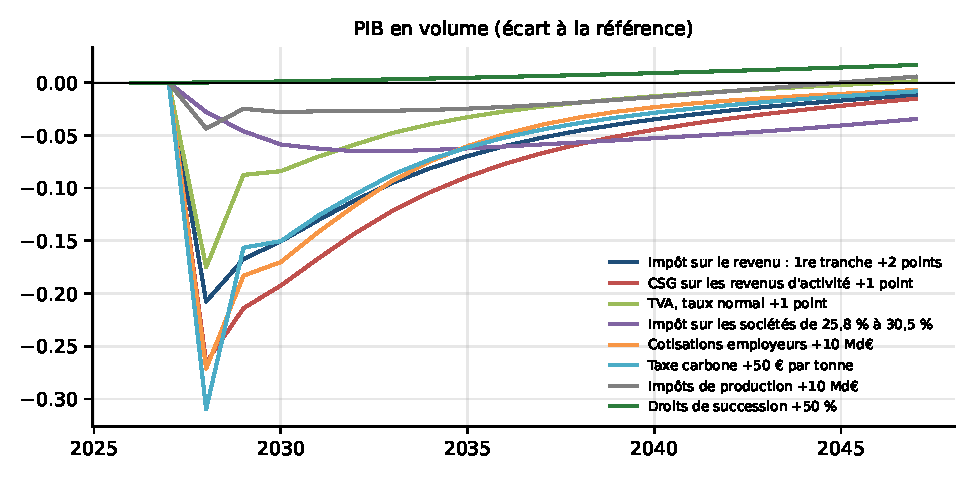
\includegraphics[width=0.95\linewidth]{pib_impots.pdf}\\
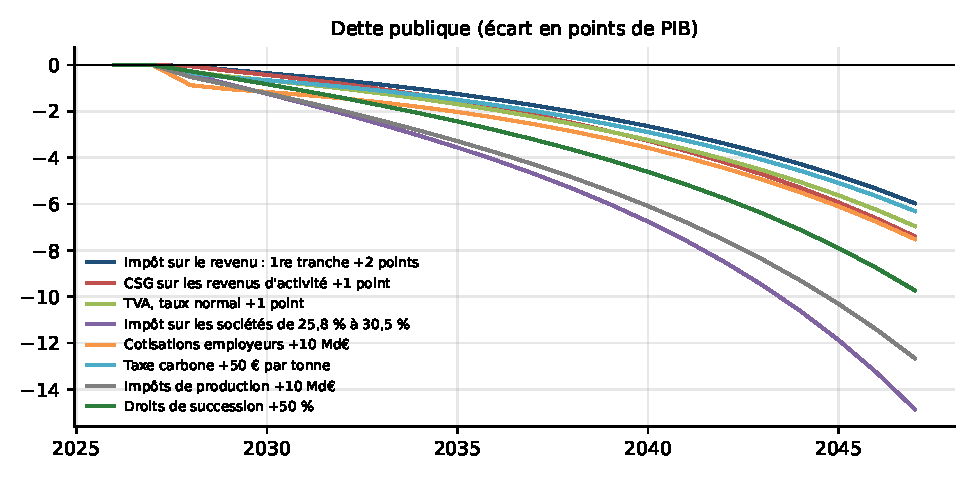
\includegraphics[width=0.95\linewidth]{dette_impots.pdf}
\caption{Expérience 1 — Trajectoires du PIB et de la dette (écarts à la référence).}
\label{fig:impots}
\end{figure}

\paragraph{Effets indirects.} \emph{Épargne} : les ménages amortissent une partie du choc en épargnant moins (taux
d'épargne $-$0,06 à $-$0,09 point pour l'IR, la CSG, l'ISF et le PFU). \emph{Investissement} : il recule avec la
demande ($-$0,2 à $-$0,3~\% pour les impôts sur les ménages) et davantage avec l'IS ($-$0,44~\%). \emph{Prix} : la
TVA et la taxe carbone relèvent les prix (+0,42~\% et +0,74~\%), les impôts sur le revenu les baissent légèrement à
moyen terme (moindre demande). \emph{Commerce extérieur} : les importations baissent avec la demande ; le solde
extérieur s'améliore légèrement. \emph{Dette} : outre le solde, le niveau des prix joue sur le ratio ; les impôts sur la
consommation, qui élèvent les prix, réduisent un peu plus le ratio de dette que les impôts sur le revenu.

\begin{figure}[htbp]
\centering
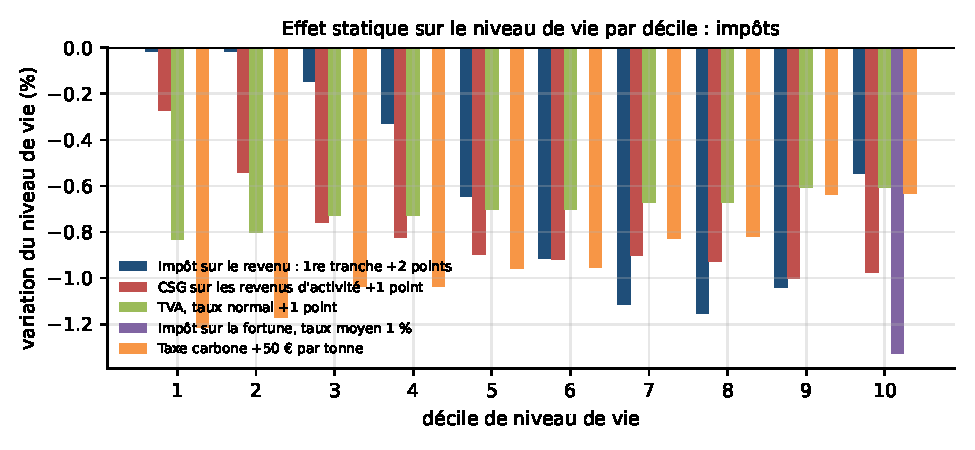
\includegraphics[width=0.9\linewidth]{distribution_impots.pdf}
\caption{Expérience 1 — Variation statique du niveau de vie par décile (microsimulation).}
\label{fig:distimpots}
\end{figure}

\paragraph{Gagnants et perdants.} (Figure~\ref{fig:distimpots}.) Les impôts sur la consommation sont
\textbf{dégressifs} par rapport au niveau de vie : la TVA retire 0,83~\% du niveau de vie du premier décile et 0,61~\% du
dernier ; la taxe carbone 1,21~\% contre 0,63~\%. Ils augmentent la pauvreté (+0,30 et +0,45 point au seuil fixe). La
CSG sur les revenus d'activité est à peu près proportionnelle au-dessus du deuxième décile (0,8 à 1~\%) et épargne en
partie les plus modestes ; elle augmente aussi la pauvreté (+0,38 point) parce qu'elle touche des travailleurs proches du
seuil. La première tranche de l'IR touche les déciles 5 à 9 ($-$0,9 à $-$1,2~\%). L'ISF et le PFU ne touchent que le
dernier décile ($-$1,3~\%) et réduisent l'indice de Gini de 0,28 point. \emph{Note} : la variation de $-$1,7~\% du premier
décile pour la tranche supérieure de l'IR est un artefact de la mesure approchée du niveau de vie (quelques foyers à
revenu fiscal élevé mais à niveau de vie calculé faible) et ne doit pas être interprétée.

\paragraph{Horizons.} L'effet sur le PIB est maximal la première année ($-$0,1 à $-$0,3~\% pour 8 à 11\md) puis
s'estompe : il est divisé par deux en cinq ans et presque nul en vingt ans, car la fermeture d'offre ramène le chômage
vers son niveau structurel. L'effet sur la dette, lui, s'accumule : $-$1,7 à $-$2,6 points en 2037, $-$6 à $-$7,5 points en
2047 pour 8 à 11\md, grâce aux intérêts économisés.

\paragraph{Conditions d'inversion.} Le solde pourrait se dégrader après une hausse d'impôt si (1) l'assiette réagit
fortement (taux marginaux élevés, contribuables mobiles : cas de la tranche supérieure de l'IR avec l'élasticité haute) ;
(2) la hausse provoque une récession durable, ce qui suppose une fermeture d'offre nulle ($\rho = 0$) \emph{et} un
multiplicateur supérieur à 1/(taux de prélèvement marginal), soit environ 2, hors de la plage du modèle ; (3) pour
l'IS, si les profits se délocalisent, ce que le modèle ne représente pas. \fiab{robuste} pour le signe de l'effet sur
le solde ; \fiab{plutôt robuste} pour l'ordre de grandeur de la perte d'activité de court terme.

\begin{resultat}
Une hausse d'impôt réduit le déficit, mais d'environ un quart à un tiers de moins que son rendement statique la
première année, à cause de l'activité perdue. Le coût en activité par euro de déficit réduit est le plus faible pour les
impôts sur le patrimoine et la TVA, le plus élevé pour la taxe carbone, les cotisations, la CSG et l'IR des classes
moyennes. Les impôts sur la consommation sont les plus défavorables aux ménages modestes.
\end{resultat}

% ====================================================================================================
\section{Expérience 2 : augmenter les salaires}
\label{sec:exp2}

\paragraph{Situation initiale.} Le salaire moyen par tête progresse d'environ 2~\% par an dans la référence ; la part des
salaires dans la valeur ajoutée est à sa norme de 2022.

\paragraph{Modifications.} Hausse générale ponctuelle de 2~\% et de 5~\% en 2028 ; « coup de pouce » au SMIC de 5~\% et
10~\% ; point d'indice de la fonction publique +3~\%.

\paragraph{Mécanismes.} Une hausse de salaire est à la fois un \emph{revenu} pour les ménages et un \emph{coût} pour les
entreprises. Dans le modèle :
\begin{enumerate}
\item le revenu des salariés augmente $\to$ consommation $\uparrow$ (effet de demande) ;
\item le coût salarial unitaire augmente $\to$ les entreprises relèvent leurs prix (0,67 la première année, tout à long
terme) $\to$ le pouvoir d'achat est en partie repris par l'inflation ;
\item le coût réel du travail augmente tant que les prix n'ont pas rattrapé $\to$ substitution du capital au travail
($\sigma = 0{,}4$) $\to$ emploi $\downarrow$ ;
\item les prix à l'exportation augmentent $\to$ perte de compétitivité-prix $\to$ exportations $\downarrow$ ;
\item les prestations sont indexées sur les prix avec retard ; les prestations sous condition de ressources (prime
d'activité, aides au logement) baissent quand le salaire augmente (effet de seuil, voir plus bas) ;
\item les recettes publiques augmentent avec la masse salariale et les prix (cotisations, TVA) ; pour le SMIC, les
allègements de cotisations indexés sur le SMIC et la masse salariale publique coûtent 0,66\md{} par point.
\end{enumerate}

\begin{table}[htbp]
\centering\scriptsize
\caption{Expérience 2 — Effets des hausses de salaires.}
\label{tab:salaires}
\tabfit{../tableaux/tab_salaires}\\[4pt]
\tabfit{../tableaux/tabd_salaires}
\end{table}

\begin{figure}[htbp]
\centering
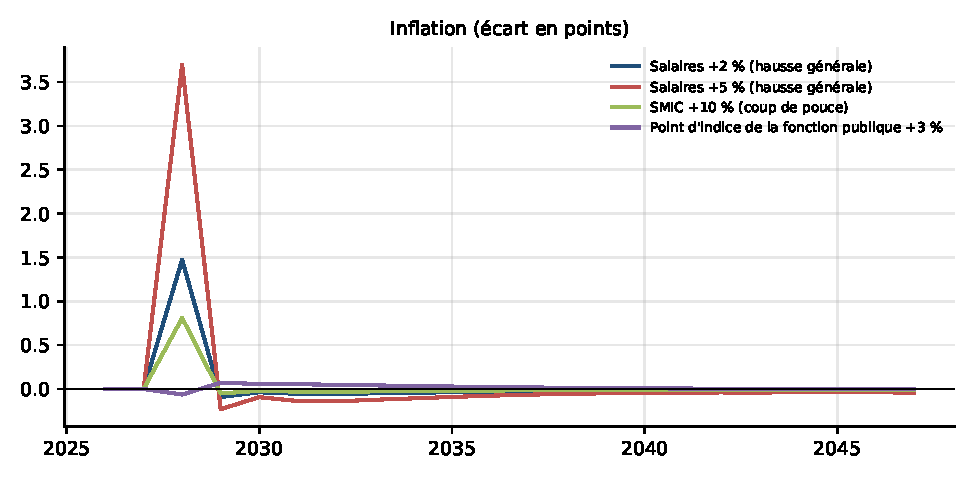
\includegraphics[width=0.48\linewidth]{inflation_salaires.pdf}\hfill
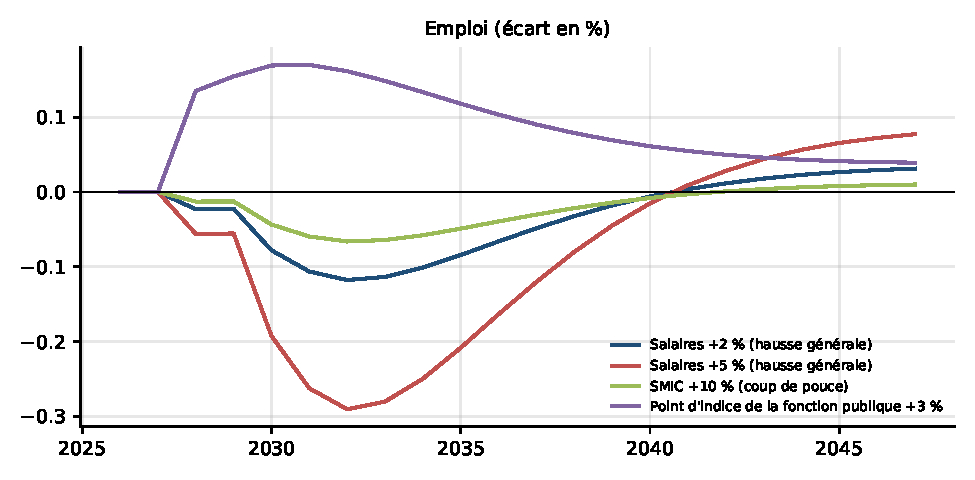
\includegraphics[width=0.48\linewidth]{emploi_salaires.pdf}
\caption{Expérience 2 — Inflation et emploi après une hausse de salaires.}
\label{fig:salaires}
\end{figure}

\paragraph{Résultats.} Une hausse générale de 2~\% en 2028 augmente le salaire moyen de 2,4~\% en 2030 (diffusion par
l'indexation), les prix de 1,3~\%, le pouvoir d'achat du revenu disponible de 0,56~\% et la consommation de 0,49~\%.
Les exportations reculent de 0,6~\%. L'emploi baisse peu la première année ($-$7\,000) puis davantage
($-$37\,000 en 2032), à mesure que la substitution capital-travail joue. Au total, le PIB est presque inchangé
(+0,02~\% en 2032) : \textbf{les effets de demande et de coût se compensent}. Le solde public s'améliore (+0,25 point en
2032) et la dette baisse de 3 à 4 points, surtout parce que l'inflation gonfle le PIB nominal et les recettes alors que
les prestations ne sont revalorisées qu'avec un an de retard. Les résultats pour +5~\% sont proportionnels.

Le \textbf{point d'indice} (+3~\%) agit comme une dépense publique : pouvoir d'achat +0,76~\%, PIB +0,22~\% en 2029,
emploi +48\,000, mais solde $-$0,25 point et dette +2,1 points en 2037.

Le \textbf{coup de pouce au SMIC} de 10~\% (diffusion supposée de 11~\% à la masse salariale) a des effets
macroéconomiques faibles : pouvoir d'achat +0,30~\%, emploi $-$21\,000 en 2032, solde $-$0,13 point (coût des allègements
indexés). \textbf{Ce résultat sous-estime probablement les pertes d'emploi peu qualifié} : le modèle n'a qu'un salaire
moyen et une élasticité de l'emploi au coût du travail commune à tous les niveaux de qualification.

\paragraph{Une hausse de salaire peut-elle augmenter la pauvreté ? Vérification par les effets de seuil.} La
microsimulation ne fait pas varier les salaires des ménages (elle est statique). Pour répondre à la question sans
présumer la réponse, le revenu disponible de trois ménages types a été calculé avec OpenFisca pour des salaires
de 0 à 2,5 SMIC (script \code{rapport/seuils\_salaires.py}, législation 2024, locataires en zone 2).

\begin{figure}[htbp]
\centering
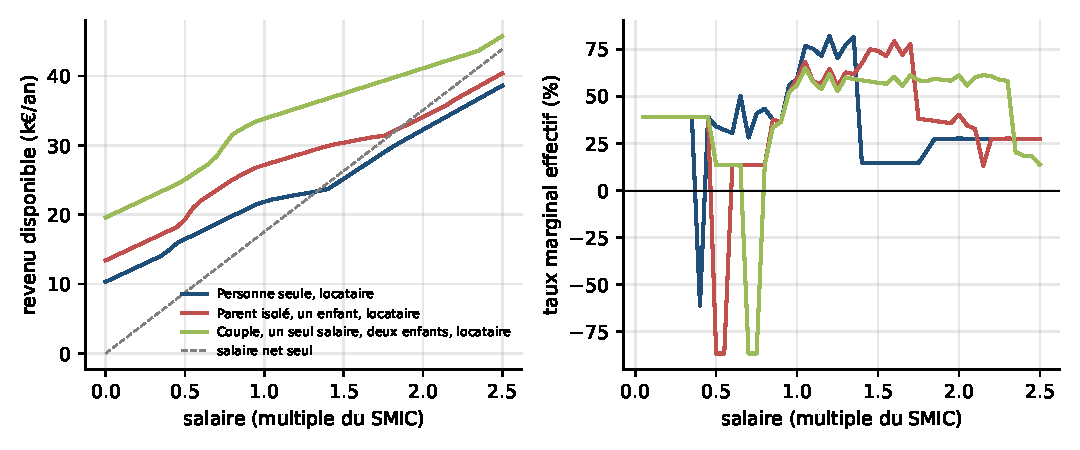
\includegraphics[width=\linewidth]{seuils_salaires.pdf}
\caption{Revenu disponible (gauche) et taux marginal effectif de prélèvement d'une hausse de salaire de 2~\% (droite)
selon le salaire, pour trois ménages types. Salaire exprimé en multiple du SMIC net imposable annuel (17\,900~€).
Revenu disponible = salaire net + RSA + prime d'activité + allocations familiales + aides au logement $-$ impôt sur le
revenu.}
\label{fig:seuils}
\end{figure}

Trois constats (figure~\ref{fig:seuils}) :
\begin{enumerate}
\item \textbf{Le revenu disponible augmente toujours avec le salaire} : il n'existe pas, dans la législation 2024 telle
qu'OpenFisca la calcule, de zone où gagner plus fait perdre du revenu disponible (pas de « trappe » au sens strict).
\item \textbf{Mais le gain est très faible entre 1 et 2 SMIC} : le taux marginal effectif atteint 55 à 82~\% (sortie
progressive de la prime d'activité et des aides au logement, entrée dans l'impôt sur le revenu). Une hausse de salaire
de 2~\% pour une personne seule au SMIC (358~€ de salaire imposable par an) ne lui rapporte que 142~€ ; pour un couple avec deux
enfants et un seul salaire, le taux marginal reste supérieur à 50~\% jusqu'à 2,2 SMIC.
\item Entre 0,3 et 0,8 SMIC, la bonification de la prime d'activité rend le taux marginal \emph{négatif} pour certains
ménages (jusqu'à $-$86~\%) : une hausse de salaire rapporte plus qu'elle-même.
\end{enumerate}

\textbf{Conclusion sur la pauvreté} : dans le modèle, une hausse de salaire \emph{n'augmente pas} la pauvreté par effet
de seuil ; elle la réduit faiblement pour les salariés modestes, car l'essentiel du gain brut est repris par la baisse
des prestations. Elle peut \emph{indirectement} toucher d'autres catégories : (1) les ménages sans revenu d'activité
(retraités, allocataires du RSA, chômeurs) subissent la hausse des prix (+1,3~\% pour +2~\% de salaires) avec un an de
retard de revalorisation ; (2) les salariés dont l'emploi est supprimé (39\,000 en 2032 pour +2~\%) ; (3) pour le SMIC,
les travailleurs peu qualifiés, dont l'emploi est probablement plus sensible au coût du travail que ne le représente
le modèle. L'ampleur de ces effets indirects sur le taux de pauvreté n'est pas mesurable avec la microsimulation
statique : \fiab{non établi}.

\paragraph{Gagnants et perdants.} Gagnants : salariés en emploi (pouvoir d'achat), administrations (inflation).
Perdants : titulaires de revenus fixes ou revalorisés avec retard (pensions, minima sociaux), salariés licenciés,
secteurs exportateurs (marges et parts de marché).

\paragraph{Horizons et inversion.} À court terme, l'effet de demande domine légèrement ; à moyen terme, l'effet de coût
(emploi $-$37\,000 à $-$92\,000 en 2032). Le résultat s'inverserait (PIB nettement négatif) si la substitution
capital-travail était forte ($\sigma = 0{,}7$) ou si les prix ne répercutaient pas les coûts (marges comprimées : emploi
$-$68\,000 pour +2~\%, contre-expertise test 5e) ; il serait plus favorable si la hausse était ciblée sur les bas
salaires des ménages à forte propension à consommer (PIB +0,13~\% en 2032, mais emploi peu qualifié non représenté).
\fiab{plutôt robuste} pour les prix et le pouvoir d'achat ; \fiab{fragile} pour l'emploi.

\begin{resultat}
Une hausse générale des salaires ne crée ni ne détruit beaucoup d'activité dans le modèle : elle redistribue vers les
salariés en emploi, au détriment des revenus fixes et de l'emploi à moyen terme. Les effets de seuil des prestations
réduisent fortement le gain net d'une hausse de salaire entre 1 et 2 SMIC (taux marginaux de 55 à 82~\%) sans créer de
perte nette de revenu disponible.
\end{resultat}

% ====================================================================================================
\section{Expérience 3 : réduire les dépenses publiques}
\label{sec:exp3}

\paragraph{Situation initiale.} Dépenses publiques : 57,3~\% du PIB en 2025, 61,5~\% en 2030 dans la référence (charge
d'intérêts, pensions).

\paragraph{Modifications.} Dix économies d'environ 10\md{} par an (ou équivalent) : 170\,000 emplois publics en moins
(en cinq ans) ; fonctionnement, santé, éducation, défense ($-$10\md{} chacun) ; investissement public ($-$10\md) ;
sous-indexation des pensions d'un point par an ; allocations chômage $-$25~\% ; prestations familiales et logement
$-$10~\% ; transferts monétaires non ciblés $-$0,3 point de PIB.

\begin{table}[htbp]
\centering\scriptsize
\caption{Expérience 3 — Effets des économies de dépenses.}
\label{tab:depenses}
\tabfit{../tableaux/tab_depenses}\\[4pt]
\tabfit{../tableaux/tabd_depenses}
\end{table}

\begin{figure}[htbp]
\centering
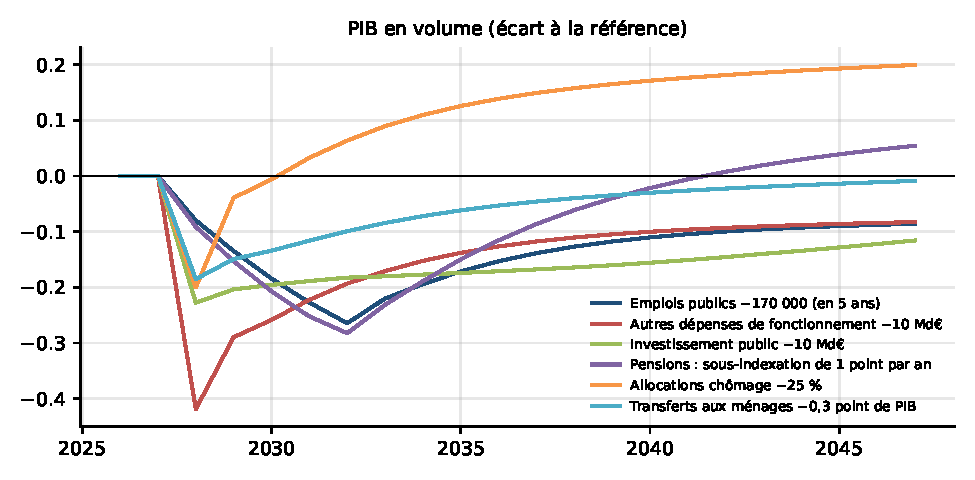
\includegraphics[width=0.95\linewidth]{pib_depenses.pdf}\\
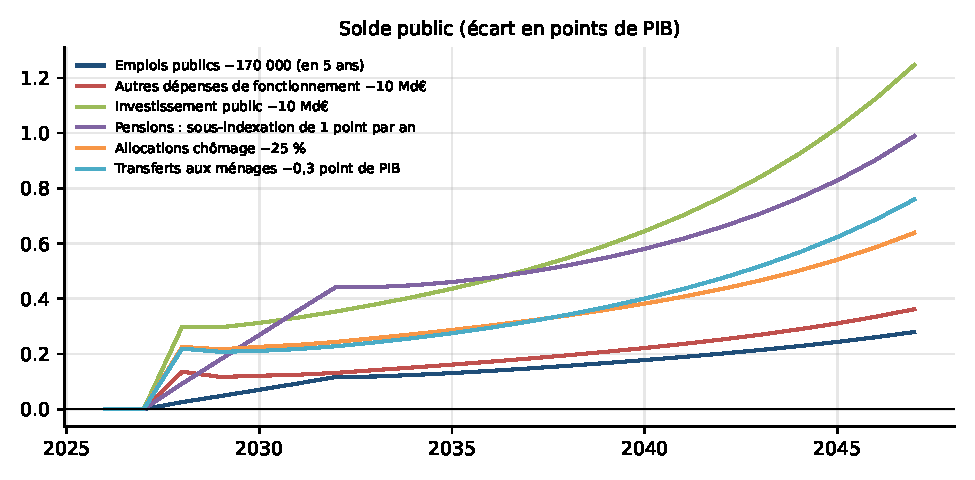
\includegraphics[width=0.95\linewidth]{solde_depenses.pdf}
\caption{Expérience 3 — PIB et solde public après différentes économies de dépenses.}
\label{fig:depenses}
\end{figure}

\paragraph{Mécanismes.} Une économie de dépense publique réduit directement la demande (achats publics, rémunérations)
ou le revenu des ménages (prestations). Deux économies de même montant diffèrent par :
\begin{enumerate}
\item \textbf{le contenu en valeur ajoutée nationale} : une dépense de fonctionnement ou un emploi public est presque
entièrement de la valeur ajoutée française ; une prestation est en partie épargnée et en partie consommée en produits
importés ; un investissement public a un contenu importé élevé (0,23 pour l'investissement contre 0,13 pour la
consommation) ;
\item \textbf{la propension à consommer des bénéficiaires} : réduire les prestations des ménages modestes réduit
davantage la consommation que réduire celles des ménages aisés ;
\item \textbf{l'effet d'offre} : seul l'investissement public améliore la capacité de production à long terme dans le
modèle ;
\item \textbf{les effets sur le marché du travail} : une baisse des allocations chômage réduit, par hypothèse, le
chômage structurel (0,1 point pour 10~\%, hypothèse \preuve{H}).
\end{enumerate}

\paragraph{Résultats.}
\begin{enumerate}
\item \textbf{Fonctionnement, santé, éducation, défense : effets identiques} ($-$0,29~\% de PIB en 2029, $-$83\,000
emplois, +0,13 point de solde en 2032). Ce n'est pas un résultat économique mais une \textbf{limite du modèle} : il ne
distingue pas ces fonctions (section~\ref{sec:depenses}). Il ne mesure ni les conséquences sur la santé, l'éducation ou
la sécurité, ni leurs effets différés sur la productivité.
\item Une économie de fonctionnement de 10\md{} n'améliore le solde que de 3,6 à 4\md{} (0,12-0,13 point de PIB) : la
moitié à deux tiers de l'économie est perdue en recettes (moindre activité) et en dépenses induites (chômage) ; c'est le
\emph{multiplicateur} de la dépense publique, proche de 1 la première année.
\item \textbf{Les économies sur les transferts sont moins coûteuses en activité} : réduire de 0,3 point de PIB
(environ 10\md) les transferts non ciblés coûte $-$0,15~\% de PIB en 2029 pour +0,21 point de solde ; la
sous-indexation des pensions $-$0,15~\% pour +0,18 point (puis +0,44 en 2032 car l'économie s'accumule) ; les
prestations familiales et de logement $-$0,06~\% pour +0,05 point.
\item \textbf{L'investissement public est l'économie la plus coûteuse à long terme} : $-$0,20~\% de PIB en 2029 mais
encore $-$0,12~\% en 2047, car le capital public se dégrade ; elle améliore pourtant fortement le solde (+0,35 point en
2032) car son contenu importé est élevé et elle n'entraîne pas de pertes de recettes importantes à court terme.
\item \textbf{La baisse des allocations chômage} ($-$25~\%) améliore le solde (+0,24 point en 2032) et, par l'hypothèse
d'effet sur le chômage structurel, augmente l'emploi à long terme (+52\,000 en 2037, PIB +0,15~\%). Sans cette
hypothèse \preuve{H}, elle n'aurait que des effets de demande négatifs.
\item La suppression de 170\,000 emplois publics en cinq ans réduit le PIB de 0,26~\% en 2032 (perte de production non
marchande), améliore peu le solde (+0,12 point) et ne réduit la dette que de 1,6 point en 2047.
\end{enumerate}

\begin{figure}[htbp]
\centering
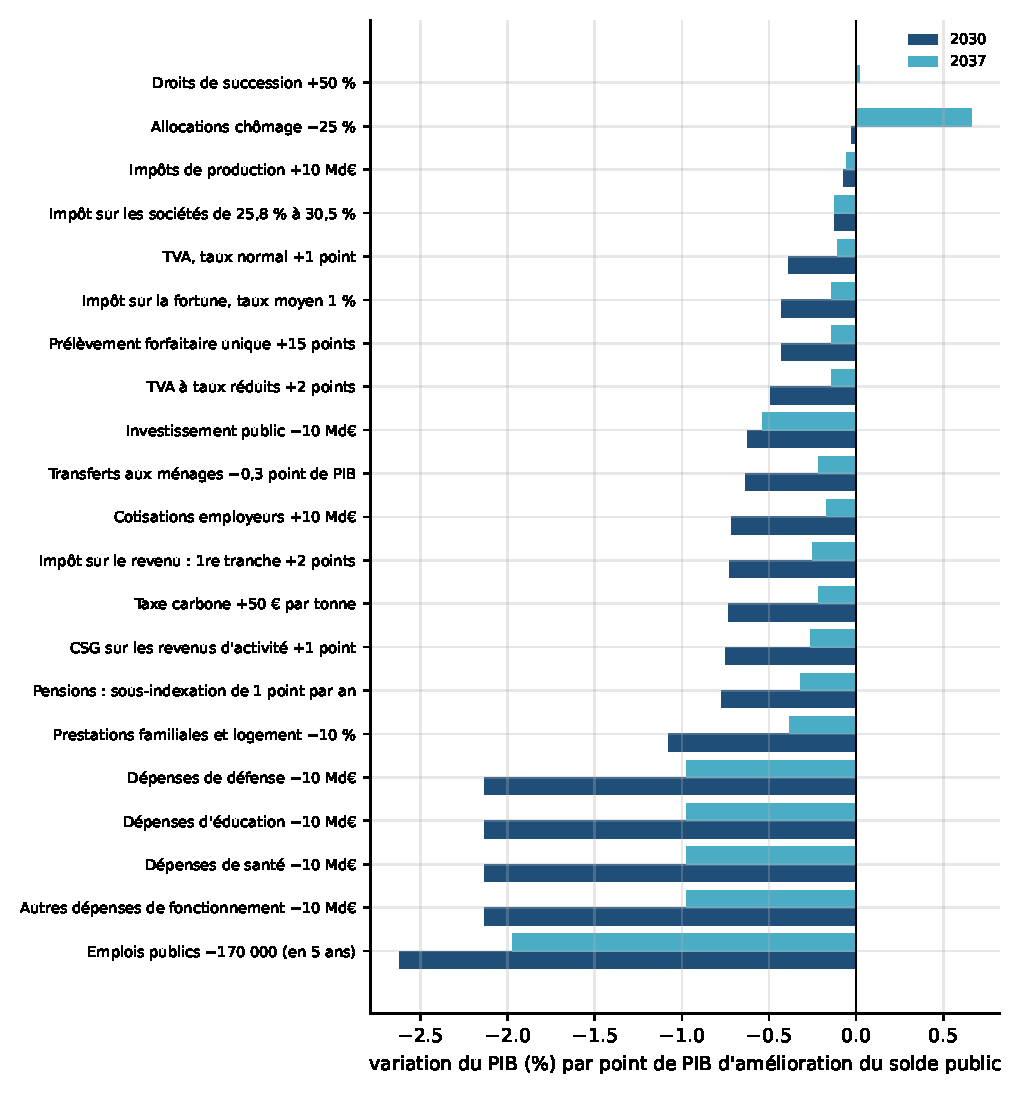
\includegraphics[width=0.9\linewidth]{efficacite_consolidation.pdf}
\caption{Coût en activité d'un point de PIB de solde public amélioré : variation du PIB (en \%) par point de PIB de
solde gagné, en 2030 et 2037. Plus la barre est à gauche, plus la mesure coûte en activité par euro de déficit réduit.}
\label{fig:efficacite}
\end{figure}

\paragraph{Pourquoi deux économies de même montant ont-elles des effets si différents ?} La
figure~\ref{fig:efficacite} classe toutes les mesures de consolidation (hausses d'impôts et baisses de dépenses) selon
leur coût en activité par point de solde gagné. Les mesures les moins coûteuses sont celles qui touchent des agents à
faible propension à dépenser en produits français (patrimoine, dividendes, transferts aux ménages aisés, IS) ; les plus
coûteuses sont celles qui réduisent directement la production nationale (emplois publics, fonctionnement) : environ
$-$2,1~\% de PIB par point de solde en 2030, contre $-$0,1 à $-$0,7 pour l'IS, la TVA ou les transferts.

\paragraph{Gagnants et perdants.} La sous-indexation des pensions touche tous les retraités (40~\% de perdants dans
chaque décile) et pèse davantage, en proportion, sur le premier décile ($-$0,93~\%) ; la baisse des prestations
familiales et de logement est très concentrée sur les deux premiers déciles ($-$2,3~\% et $-$1,4~\%) et augmente la
pauvreté de 0,42 point. Les économies de fonctionnement et d'emplois publics touchent les usagers des services publics,
dont la valeur n'est pas mesurée par le modèle.

\paragraph{Horizons et inversion.} L'effet récessif est maximal la première année et s'estompe ; l'économie budgétaire
s'accumule en dette évitée. Le classement des mesures pourrait changer si l'on représentait l'effet des dépenses
d'éducation, de santé et de recherche sur la productivité : ces dépenses deviendraient alors plus coûteuses à réduire à
long terme. \fiab{plutôt robuste} pour le classement de court terme ; \fiab{non établi} pour les effets de long terme des
dépenses autres que l'investissement.

\begin{resultat}
À montant égal, une économie sur les transferts monétaires coûte trois à sept fois moins d'activité, par point de
déficit réduit, qu'une économie sur la production publique (emplois, fonctionnement). Mais le modèle ignore la valeur
des services publics et leurs effets de long terme : il ne peut pas dire quelles dépenses sont « inefficaces ».
\end{resultat}

% ====================================================================================================
\section{Expérience 4 : réduire les cotisations sociales}
\label{sec:exp4}

\paragraph{Situation initiale.} Les cotisations sociales représentent environ 17~\% du PIB de recettes ; les allègements
généraux sur les bas salaires coûtent environ 80\md{} par an.

\paragraph{Modifications.} Baisse des cotisations employeurs de 10\md{} et 20\md{} par an, non compensée ; puis
« TVA sociale » : baisse de 20\md{} financée par une hausse de 2,4 points du taux normal de TVA.

\begin{table}[htbp]
\centering\scriptsize
\caption{Expérience 4 — Baisse des cotisations employeurs.}
\label{tab:cotisations}
\tabfit{../tableaux/tab_cotisations}\\[4pt]
\tabfit{../tableaux/tabd_cotisations}
\end{table}

\paragraph{Mécanismes.} La baisse des cotisations réduit le coût du travail $\to$ (1) les entreprises baissent leurs
prix (0,67 de la baisse du coût unitaire la première année) $\to$ pouvoir d'achat et compétitivité-prix
$\uparrow$ ; (2) le coût réel du travail baisse $\to$ substitution en faveur du travail ; (3) la recette publique
diminue. À moyen terme, le salaire brut s'ajuste : la part des salaires dans la valeur ajoutée revient vers sa norme,
si bien qu'une partie de la baisse de cotisations est captée par des hausses de salaires.

\paragraph{Résultats.} Une baisse de 20\md{} augmente le PIB de 0,36~\% en 2029, l'emploi de 86\,000 puis 109\,000 en
2032, abaisse les prix de 0,77~\% et augmente le pouvoir d'achat de 0,89~\%. Les exportations progressent de 0,38~\%.
Elle coûte 0,47 point de PIB de solde en 2029 et 0,51 en 2032 (soit 70~\% de son coût statique : 30~\% est
autofinancé par l'activité), et la dette augmente de 5 points en 2037. L'effet s'estompe : PIB +0,08~\% en 2037,
emploi +53\,000 ; il est presque nul en 2047. \textbf{Le salaire moyen baisse de 1,3~\% en 2030 par rapport à la
référence} : c'est l'effet de la baisse des prix sur l'indexation et du ralentissement des salaires ; en termes
réels, le pouvoir d'achat augmente.

La \textbf{TVA sociale} combine les deux effets : PIB +0,15~\% en 2029 (+0,09 en 2032), emploi +30\,000 à +50\,000,
solde quasiment neutre (+0,03 à +0,08 point). Elle transfère la charge du coût du travail vers la consommation : les
prix augmentent de 0,23~\% puis 0,54~\%, et les ménages modestes et les retraités paient davantage (pauvreté +0,79 point
dans la microsimulation, qui ne voit que la hausse de TVA et pas les éventuels effets sur les salaires).

\paragraph{Gagnants et perdants.} Baisse non financée : entreprises (marges), salariés (emploi, pouvoir d'achat par la
baisse des prix) ; perdants : les finances publiques, donc les contribuables futurs. TVA sociale : gagnants : salariés
et entreprises exportatrices ; perdants : retraités, allocataires de minima, ménages modestes.

\paragraph{Horizons et inversion.} Les effets sur l'emploi sont plus importants à moyen terme (2030-2032) qu'à court
terme, puis s'estompent quand les salaires s'ajustent. \textbf{Le modèle sous-estime probablement l'effet d'une baisse
ciblée sur les bas salaires}, où l'emploi réagit davantage au coût du travail (littérature sur les allègements) ; il
surestime peut-être celui d'une baisse uniforme sur les hauts salaires. \fiab{plutôt robuste} pour le signe ;
\fiab{fragile} pour l'ampleur de l'emploi (élasticité de substitution calibrée).

% ====================================================================================================
\section{Expérience 5 : stimuler l'investissement productif}
\label{sec:exp5}

\paragraph{Modifications.} Investissement public +10\md{} et +30\md{} par an ; baisse de l'IS de 25,8~\% à 20~\%
(incitation à l'investissement privé) ; construction de 50\,000 logements sociaux supplémentaires par an.

\begin{table}[htbp]
\centering\scriptsize
\caption{Expérience 5 — Investissement public et privé.}
\label{tab:invest}
\tabfit{../tableaux/tab_investissement}\\[4pt]
\tabfit{../tableaux/tabd_investissement}
\end{table}

\begin{figure}[htbp]
\centering
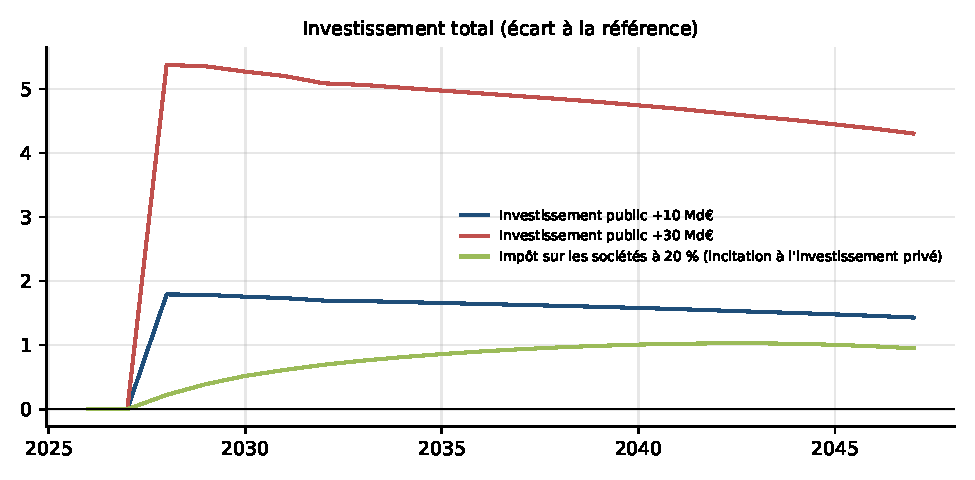
\includegraphics[width=0.85\linewidth]{fbcf_invest.pdf}
\caption{Expérience 5 — Investissement total (écart à la référence).}
\end{figure}

\paragraph{Mécanismes.} L'investissement public agit de deux façons : à court terme comme une demande (avec un
contenu importé élevé, 23~\%), à long terme par l'accumulation d'un capital public qui rend le secteur privé plus
productif (élasticité 0,08). La baisse de l'IS réduit le coût du capital et augmente l'investissement des entreprises
d'environ 1,2~\% à long terme ; une partie des profits libérés est distribuée (50~\%), dont 30~\% à l'étranger.

\paragraph{Résultats.} \textbf{L'investissement public est le seul levier de dépense dont l'effet sur le PIB persiste} :
+10\md{} par an donnent +0,20~\% de PIB en 2029, encore +0,17~\% en 2037 et +0,12~\% en 2047 ; +30\md{} donnent
+0,61~\%, +0,50~\% et +0,35~\%. Il ne s'autofinance pas : 10\md{} dégradent le solde de 0,30 point en 2029 (90~\% de son
coût) et la dette de 10,5 points en 2047. L'emploi augmente à court terme (+24\,000) puis l'effet s'annule : à long terme,
le gain de PIB vient de la productivité, pas de l'emploi. Les importations augmentent de 0,49~\% : un quart de la
dépense « fuit » à l'étranger.

La \textbf{baisse de l'IS} à 20~\% a des effets faibles mais durables : investissement +0,52~\% en 2030, PIB +0,05 à
+0,08~\%, emploi +8\,000 à +18\,000 ; elle coûte 0,56 à 0,63 point de PIB de solde (17 à 19\md) et 19 points de dette en
2047. \fiab{robuste} pour le faible effet, dans le cadre du modèle ; la littérature internationale trouve des effets
plus forts quand on tient compte de la localisation des investissements et des profits.

Les \textbf{logements sociaux} (50\,000 par an, subvention publique de 25~\%) augmentent l'investissement de 1,5~\% et
le PIB de 0,17~\% en 2029 pour un coût budgétaire presque nul ; mais le modèle ne représente ni les loyers, ni la
mobilité, ni le financement par emprunt des bailleurs (\fiab{fragile}).

\paragraph{Investissements productifs et dépenses qui ne le sont pas.} Dans le modèle, la distinction se fait par un seul
paramètre : l'élasticité de la production au capital public (0,08, plage 0,04-0,12 ; 0,12 pour les infrastructures).
Une dépense sans effet d'offre (fonctionnement) a un effet sur le PIB qui disparaît en dix ans ; un investissement public
avec effet d'offre garde un tiers à la moitié de son effet initial au bout de vingt ans. Avec l'élasticité basse (0,04),
l'effet de long terme est divisé par deux ; avec la haute (0,12), il augmente de moitié.

\paragraph{Gagnants et perdants.} Investissement public : entreprises du BTP et de l'équipement, utilisateurs des
infrastructures ; coût porté par la dette. Baisse d'IS : actionnaires (dont 30~\% non résidents), entreprises
capitalistiques.

\paragraph{Conditions d'inversion.} Si l'investissement public est mal choisi (élasticité nulle), il devient une
dépense comme une autre ; si les taux d'intérêt montent fortement en réaction à la dette, l'effet d'éviction réduit le
gain (avec la prime de risque, déjà incluse : +3 points de base par point de dette).

% ====================================================================================================
\section{Expérience 6 : réindustrialiser la France}
\label{sec:exp6}

\paragraph{Situation initiale.} L'industrie manufacturière représente 9,6~\% du PIB en 2025 et continue de reculer dans la
référence. Le contenu en importations est élevé dans la chimie, la pharmacie, la métallurgie, l'électronique, les
équipements électriques, les machines et l'automobile.

\paragraph{Modifications.} Objectif de substitution d'importations : $-$10~\% et $-$20~\% des parts importées de huit produits
industriels, atteint en cinq ans après deux ans de construction des usines, avec un investissement de capacité
(ratio capital / valeur ajoutée de chaque branche) et un surcoût de production de 10~\% par rapport aux importations.
Variantes : avec une énergie importée plus chère de 20~\% ; avec des droits de douane de 10~\% sur les importations hors
Union européenne (et riposte des partenaires) ; droits de douane seuls.

\begin{table}[htbp]
\centering\scriptsize
\caption{Expérience 6 — Réindustrialisation et protection commerciale.}
\label{tab:industrie}
\tabfit{../tableaux/tab_industrie}\\[4pt]
\tabfit{../tableaux/tabd_industrie}
\end{table}

\begin{figure}[htbp]
\centering
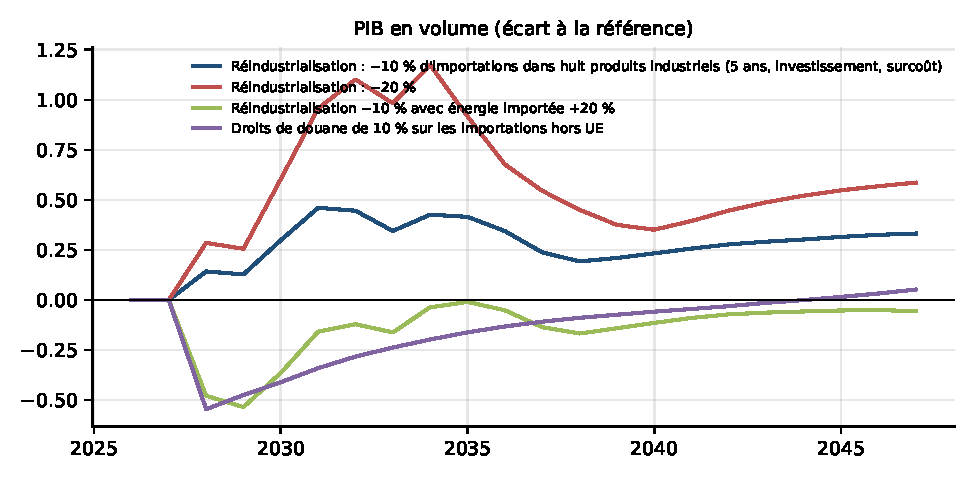
\includegraphics[width=0.95\linewidth]{pib_industrie.pdf}\\
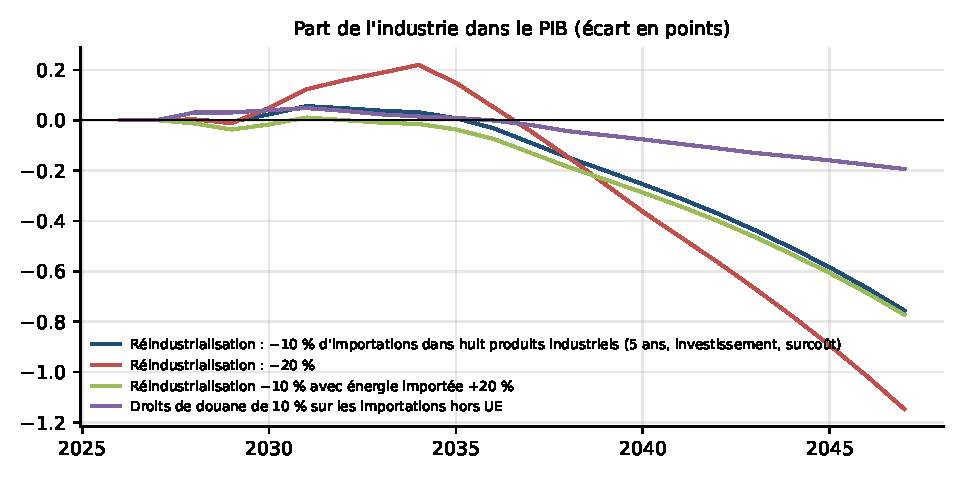
\includegraphics[width=0.95\linewidth]{industrie_part.pdf}
\caption{Expérience 6 — PIB et part de l'industrie dans le PIB.}
\label{fig:industrie}
\end{figure}

\paragraph{Mécanismes.} Produire en France ce qui était importé (1) remplace des importations par de la production
nationale (valeur ajoutée, emplois, revenus, recettes) ; (2) exige d'abord un investissement de capacité (demande
supplémentaire pendant la construction) ; (3) renchérit les produits concernés (surcoût de 10~\%), ce qui se propage aux
prix ; (4) mobilise de la main-d'œuvre, ce qui tend le marché du travail et les salaires.

\paragraph{Résultats.} Une relocalisation de 10~\% augmente le PIB de 0,45~\% en 2032 et l'emploi de 80\,000 ; 20~\%
donne +1,10~\% et +179\,000. L'investissement augmente de 1 à 2~\% pendant la construction. Les prix augmentent de 0,4 à
1,1~\% en 2037 (surcoût). Le solde public s'améliore un peu (+0,17 à +0,37 point en 2032). La part de l'industrie dans le
PIB ne gagne que 0,05 à 0,16 point : \textbf{une relocalisation de 10 à 20~\% des importations de huit produits ne
change pas l'ordre de grandeur du poids de l'industrie}. Après la phase de construction, l'effet sur le PIB diminue
(+0,24~\% en 2037 pour 10~\%) car l'investissement de capacité retombe et le surcoût pèse sur le pouvoir d'achat.

\textbf{Avec une énergie importée plus chère de 20~\%}, la même relocalisation donne un PIB inférieur à la référence
($-$0,54~\% en 2029, $-$0,12~\% en 2032) et une dette plus élevée de 26 points en 2047 : le choc énergétique annule le
gain de la relocalisation. \textbf{Les droits de douane de 10~\%}, avec riposte, réduisent le PIB de 0,47~\% en 2029
(exportations $-$3,3~\%, prix +1,2~\%) ; combinés à la relocalisation, ils en annulent le bénéfice (PIB $-$1,04~\% en
2029, $-$0,45~\% en 2032) : la protection commerciale fait payer aux exportateurs et aux consommateurs ce qu'elle
apporte aux producteurs protégés.

\paragraph{Ce que le modèle ne dit pas.} La relocalisation est ici un \textbf{objectif imposé}, pas le résultat d'une
politique : le modèle ne dit pas comment l'atteindre (aides, compétitivité, énergie, foncier), ni si les qualifications
nécessaires existent (pas de contrainte de main-d'œuvre par métier), ni quelles matières et quels composants seraient
alors importés (dépendances matérielles représentées en valeur seulement). \fiab{fragile} : le résultat est
proportionnel à l'hypothèse de substitution.

\paragraph{Gagnants et perdants.} Gagnants : salariés et territoires industriels, finances publiques ; perdants :
consommateurs des produits relocalisés (surcoût), et, avec des droits de douane, les exportateurs et les ménages
modestes (hausse des prix).

\paragraph{Conditions d'inversion.} Énergie chère, surcoût supérieur à 20~\%, droits de douane avec riposte, ou
relocalisation financée par des aides publiques non chiffrées ici.

% ====================================================================================================
\section{Expérience 7 : modifier les prestations sociales}
\label{sec:exp7}

\paragraph{Modifications.} RSA +25~\% ; prime d'activité +25~\% ; allocations familiales +25~\% ; aides au logement
$-$10~\% ; minimum vieillesse +25~\%.

\begin{table}[htbp]
\centering\scriptsize
\caption{Expérience 7 — Prestations sociales.}
\label{tab:prestations}
\tabfit{../tableaux/tab_prestations}\\[4pt]
\tabfit{../tableaux/tabd_prestations}
\end{table}

\begin{figure}[htbp]
\centering
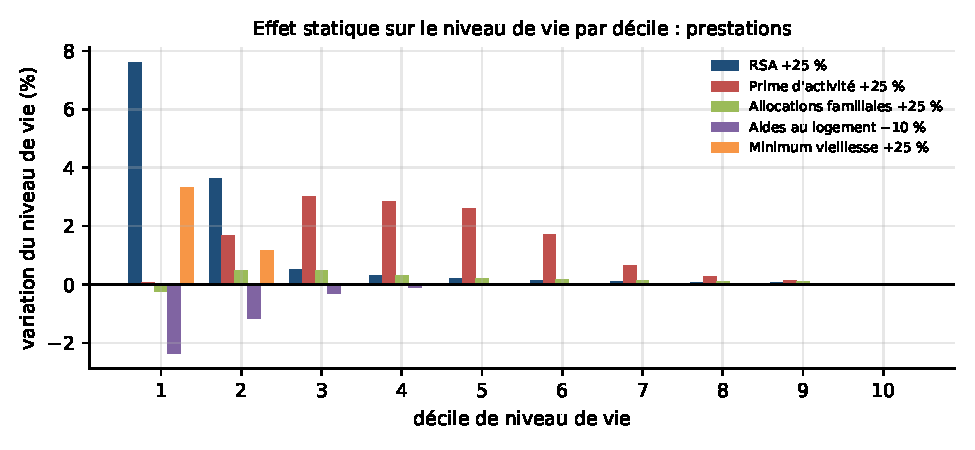
\includegraphics[width=0.9\linewidth]{distribution_prestations.pdf}
\caption{Expérience 7 — Variation statique du niveau de vie par décile.}
\label{fig:distprest}
\end{figure}

\paragraph{Mécanismes.} Une prestation sous condition de ressources augmente le revenu de ménages modestes à forte
propension à consommer $\to$ consommation $\uparrow$ ; elle coûte au budget ; elle modifie les incitations au travail par
le taux marginal effectif (figure~\ref{fig:seuils}).

\paragraph{Résultats.} \textbf{La prime d'activité est le levier le plus efficace contre la pauvreté par euro dépensé
dans le modèle} : +25~\% réduit la pauvreté de 1,43 point (statique) pour un coût de 0,24 point de PIB de solde ; elle
profite aux déciles 2 à 6 (+1,7 à +3~\%). Le RSA +25~\% réduit la pauvreté de 0,33 point et l'indice de Gini de 0,38
point, pour un coût plus faible (0,09 point de PIB) ; il profite au premier décile (+7,6~\%). Les allocations familiales
+25~\% réduisent la pauvreté de 0,55 point ; une partie des ménages du premier décile y perdent (10~\%) parce que les
allocations familiales entrent dans la base ressources du RSA et de la prime d'activité : c'est une interaction entre
barèmes, dont l'ampleur dépend des hypothèses de recours. Le minimum vieillesse +25~\% améliore le niveau de vie des deux
premiers déciles de 3,3 et 1,2~\% pour un coût faible. La baisse des aides au logement de 10~\% augmente la pauvreté de
0,18 point et touche le premier décile ($-$2,4~\%). Effets macroéconomiques : faibles et positifs (PIB +0,03 à +0,25~\%
en 2029), s'estompant à long terme.

\paragraph{Incitations au travail.} Le modèle ne représente pas la réaction de l'offre de travail aux prestations (pas
d'élasticité de participation) : une hausse du RSA, qui augmente le revenu sans emploi, et une hausse de la prime
d'activité, qui augmente le gain à l'emploi, n'ont pas d'effet différent sur l'emploi. Les taux marginaux effectifs de
la figure~\ref{fig:seuils} montrent qu'une hausse de la prime d'activité améliore l'incitation à reprendre un emploi à
temps partiel, mais prolonge la zone de taux marginaux élevés entre 1 et 2 SMIC. \fiab{non établi}.

\paragraph{Conditions d'inversion.} Le non-recours (un tiers des ayants droit au RSA et à la prime d'activité) réduit
l'effet sur la pauvreté ; une réaction négative de l'offre de travail au RSA réduirait son efficacité.

% ====================================================================================================
\section{Expérience 8 : augmenter le temps de travail}
\label{sec:exp8}

\paragraph{Modifications.} Durée légale du travail portée à 37 heures, ou abaissée à 32 heures (mise en place en deux
ans) ; âge légal de départ en retraite porté progressivement à 65 ou 66 ans, ou ramené à 62 ans (trois mois par
génération).

\begin{table}[htbp]
\centering\scriptsize
\caption{Expérience 8 — Durée du travail et âge de départ.}
\label{tab:travail}
\tabfit{../tableaux/tab_travail}\\[4pt]
\tabfit{../tableaux/tabd_travail}
\end{table}

\begin{figure}[htbp]
\centering
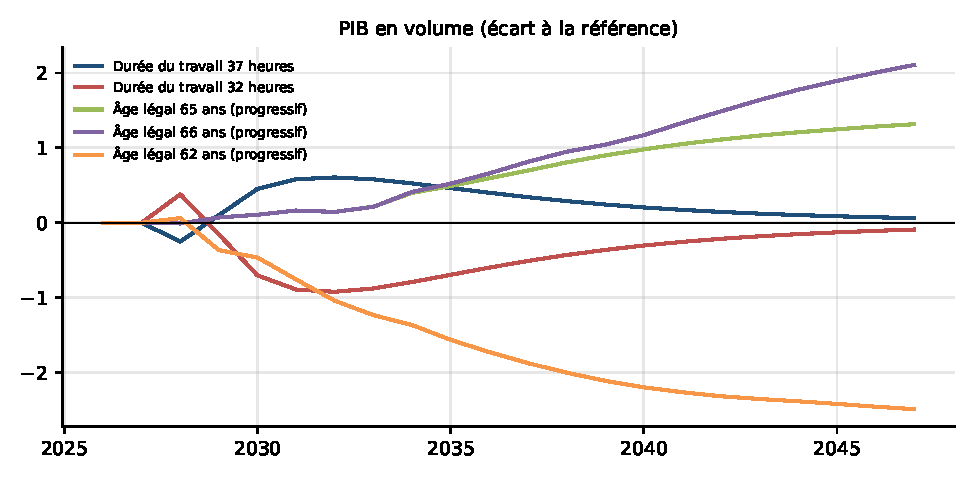
\includegraphics[width=0.95\linewidth]{pib_travail.pdf}\\
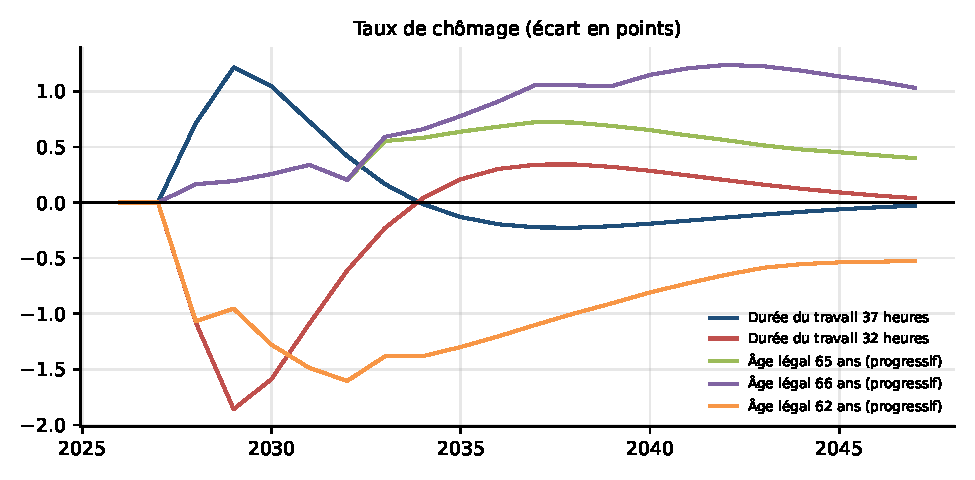
\includegraphics[width=0.95\linewidth]{chomage_travail.pdf}
\caption{Expérience 8 — PIB et chômage.}
\label{fig:travail}
\end{figure}

\paragraph{Mécanismes.} \emph{Durée hebdomadaire} : le modèle suppose que 70~\% d'une variation des heures est absorbée
sans changement d'effectif (productivité horaire, intensité, heures supplémentaires) et que les salaires mensuels sont
maintenus \preuve{H, calé sur l'ordre de grandeur des 35 heures}. Allonger la durée augmente donc la production par
salarié : les entreprises ont besoin de moins de salariés pour la même production, le coût horaire baisse. \emph{Âge de
départ} : plus d'actifs (offre de travail), moins de pensions ; les seniors maintenus actifs sont en emploi à 89~\%
la première année, mais l'économie doit créer les emplois correspondants (fermeture d'offre).

\paragraph{Résultats.} \textbf{37 heures} : la production par tête augmente, mais \textbf{l'emploi baisse fortement à
court terme} ($-$408\,000 en 2029, chômage +1,05 point) parce que la demande ne suit pas immédiatement l'offre ; la baisse
du coût horaire réduit les prix ($-$1,25~\%) et soutient les exportations (+0,9~\%) ; le PIB augmente (+0,60~\% en 2032)
à mesure que la fermeture d'offre résorbe le chômage ; en 2037, l'emploi redevient supérieur à la référence (+76\,000).
\textbf{32 heures} : effet inverse, emploi +624\,000 en 2029 (partage du travail), chômage $-$1,6 point, mais PIB
$-$0,92~\% en 2032, prix +2~\% et exportations $-$1,3~\% ; à long terme, l'emploi devient inférieur à la référence.

\textbf{Âge de départ à 65 ans} : le PIB augmente lentement (+0,14~\% en 2032, +0,70~\% en 2037, +1,31~\% en 2047) avec la
population active ; le chômage augmente d'abord (+0,26 point en 2030), le temps que l'emploi rattrape ; 66 ans : +2,1~\%
de PIB en 2047. \textbf{Retour à 62 ans} : PIB $-$1,04~\% en 2032, $-$2,5~\% en 2047 ; emploi $-$570\,000 en 2037 ; le chômage
baisse (moins d'actifs) ; les pensions augmentent.

Un résultat contre-intuitif mérite d'être signalé : \textbf{le report de l'âge à 65 ans n'améliore presque pas le
ratio de dette dans le modèle} (+0,9 point en 2047 alors que le solde s'améliore de 0,16 à 0,18 point). L'afflux
d'actifs augmente d'abord le chômage, ce qui modère les salaires et les prix ($-$0,9~\% en 2037) : le PIB nominal, au
dénominateur du ratio, est plus bas. Ce mécanisme de prix est \fiab{fragile} (courbe de Phillips calibrée) ; l'effet sur
les pensions (moins de pensions versées) est \fiab{robuste}.

\paragraph{Gagnants et perdants.} 37 heures : salariés en emploi (même salaire, plus d'heures : baisse du salaire
horaire), entreprises ; perdants : chômeurs supplémentaires à court terme. Report de l'âge : finances sociales et
actifs futurs ; perdants : générations concernées (carrières plus longues, en particulier les métiers pénibles, non
distingués dans le modèle).

\paragraph{Conditions d'inversion.} Si l'économie absorbe les actifs supplémentaires plus vite (fermeture forte), le
gain de PIB du report de l'âge arrive plus tôt ; si elle ne les absorbe pas (fermeture nulle), le report augmente
durablement le chômage. La contre-expertise donne, pour un retour à 62 ans, une plage de $-$2,4~\% à +0,3~\% de PIB en
2032 : \fiab{fragile}. Pour la durée hebdomadaire, tout dépend de l'hypothèse de compensation (70~\%), qui n'est pas
estimée : \fiab{fragile}.

\begin{resultat}
Travailler plus (durée ou carrière) augmente la production à long terme, mais pas immédiatement : à court terme,
l'économie doit créer les emplois correspondants, et le chômage augmente d'abord. Réduire le temps de travail partage
l'emploi existant à court terme mais réduit la production et la compétitivité.
\end{resultat}
